\chapter[Metodologia]{Metodologia}

\section{Metodologia de Desenvolvimento de Software}

Um processo ou metodologia de desenvolvimento de software é uma coleção de atividades e resultados relacionados que auxiliam na criação de software. Por exemplo, análise e codificação de requisitos são duas das muitas atividades associadas. \cite{Soares2004}

Há vários tipos de metodologia de desenvolvimento de software como o Scrum, PMBOK, Kanban, Ágil, Ciclo de Vida Único, Modelo em cascata, entre outras. Cada uma delas possui suas próprias características e abordagens para gerenciamento de projetos, mas todas elas visam ajudar as equipes a entregar projetos de software de qualidade dentro do prazo, orçamento e com as funcionalidades esperadas. Algumas metodologias são mais estruturadas e baseadas em fases, enquanto outras são mais flexíveis e baseadas em fluxo de trabalho, o que torna importante escolher a metodologia mais adequada para o projeto específico. \cite{SilvaAnd2013}

\subsection{Metodologia Ágil}

As metodologias ágeis são um conjunto de abordagens para gerenciamento de projetos que se concentram em fornecer flexibilidade, adaptabilidade e colaboração entre equipes. Elas foram desenvolvidas originalmente para o desenvolvimento de software, mas agora são amplamente utilizadas em muitos outros campos. \cite{Libardi2010}

\subsubsection{Scrum}

Scrum é uma metodologia ágil específica que foi projetada para ajudar equipes a gerenciar projetos de desenvolvimento de software complexos e altamente incertos. Ele se concentra em entregar valor rapidamente e incrementos regulares, enquanto a equipe colabora e se adapta a mudanças no projeto. \cite{STOPA2019}

\subsubsection{Kanban}

Kanban é uma metodologia que se concentra em tornar visível o fluxo de trabalho, limitando o número de tarefas em andamento e permitindo que a equipe se adapte às mudanças de forma flexível. Ele é amplamente utilizado em conjunto com outras metodologias ágeis, como Scrum, para ajudar a equipe a aumentar a eficiência e a entrega de valor. \cite{Lage2008}

\subsection{Metodologia de Desenvolvimento Utilizada}

Kanban e Scrum são ambas metodologias ágeis, mas possuem abordagens diferentes para o gerenciamento de projetos. Enquanto o Scrum é uma metodologia mais estruturada e baseada em sprints, Kanban é uma metodologia mais flexível e baseada no fluxo de trabalho. Ambos têm seus próprios benefícios e podem ser usados de forma complementar para ajudar a equipe a alcançar seus objetivos de projeto. \cite{Kniberg2010}

Sendo assim, o projeto foi desenvolvido utilizando ambas as metodologias, Kanban e Scrum, para que fosse possível atingir os objetivos propostos. O Kanban foi utilizado para gerenciar o fluxo de trabalho, enquanto o Scrum foi utilizado para gerenciar as sprints.

\section{Ferramentas Utilizadas}

\subsection{Gerenciamento do Projeto}

\subsubsection{Trello}

Trello é uma plataforma que auxilia equipes a organizarem e priorizarem projetos. Utiliza quadros de tarefas, onde cada tarefa é representada por um cartão, que pode ser movido e organizado em listas para indicar o progresso e o estado do projeto. Ele é uma ferramenta útil para gerenciar tarefas do projeto, estabelecer prazos e definir prioridades, além de acompanhar o andamento de cada Sprint.

\subsubsection{Slack}

Slack é uma ferramenta de comunicação de equipe que permite que as equipes criem canais de bate-papo para discutir projetos, compartilhar arquivos e se comunicar de forma rápida e eficiente.

No contexto do desenvolvimento de software, Slack pode ajudar a equipe a se comunicar de forma mais eficiente e colaborativa, permitindo que desenvolvedores, gerentes de projetos e outros membros da equipe discutam e compartilhem informações de forma rápida e fácil. Ele pode ser usado para discutir problemas técnicos, atribuir tarefas, acompanhar o progresso do projeto e compartilhar arquivos, tudo em um único lugar. Além disso, ele pode ser integrado com outras ferramentas, como o GitHub, o Google Drive e o Trello, para ajudar a equipe a automatizar tarefas e trabalhar de forma mais eficiente.

\subsubsection{Google Drive}

Google Drive é um serviço de armazenamento e compartilhamento de arquivos na nuvem fornecido pelo Google. Ele permite que os usuários armazenem arquivos, como documentos, fotos e vídeos, e compartilhem esses arquivos com outras pessoas. Ele também oferece recursos de colaboração, como edição em tempo real de documentos, comentários e histórico de versões.

\subsection{Desenvolvimento}

\subsubsection{Figma}

Figma é uma ferramenta de design colaborativo que permite que equipes criem e compartilhem arquivos de design. Ele permite que os usuários criem protótipos de aplicativos e sites, além de permitir que eles compartilhem esses protótipos com outras pessoas para que possam colaborar e fazer comentários. Ele também permite que os usuários criem e compartilhem arquivos de design, como imagens, ícones e paletas de cores, que podem ser usados por outros membros da equipe.

\subsubsection{GitHub e GitHub Actions}

GitHub é uma plataforma de desenvolvimento de software que permite que os desenvolvedores armazenem, rastreiem e colaborem em projetos de código-fonte. Ele é baseado no sistema de controle de versão Git, que permite que os desenvolvedores façam alterações no código e versionem essas alterações, facilitando a colaboração e o controle de versão.

GitHub Actions é uma ferramenta de automação de fluxo de trabalho do GitHub. Ele permite que os desenvolvedores criem scripts de trabalho automatizados, chamados "Ações", que podem ser disparados por eventos, como o envio de código para o repositório ou a criação de uma nova issue. Isso permite automatizar tarefas comuns, como compilação, teste e implantação, e integrar com outras ferramentas, como ferramentas de integração contínua e de monitoramento de desempenho.

\subsubsection{Docker}

Docker é uma plataforma de virtualização de aplicativos que permite que os desenvolvedores embalem e distribuam facilmente aplicativos em contêineres. Um contêiner é uma forma de isolamento de sistemas operacionais que permite que um aplicativo seja embalado com todas as suas dependências, bibliotecas e configurações, de forma que possa ser executado de forma consistente em diferentes ambientes.

Docker permite que os desenvolvedores criem e gerenciem contêineres, e que esses contêineres sejam implantados em diferentes ambientes, incluindo computadores locais, nuvens públicas e privadas. Isso permite que os desenvolvedores criem aplicativos de forma mais eficiente e confiável, e que esses aplicativos possam ser executados de forma consistente em diferentes ambientes. Além disso, ele também permite a colaboração entre equipes, e aumenta a segurança, escalabilidade e gerenciamento do aplicativo.

\subsubsection{Visual Studio Code}

VSCode (Visual Studio Code) é um editor de código-fonte desenvolvido pela Microsoft. Ele é uma ferramenta gratuita e de código aberto, que suporta diversas linguagens de programação, incluindo JavaScript, Python, C++, Java e muitas outras. Ele oferece recursos avançados de edição, como sugestão de código, depuração e gerenciamento de versão. Além disso, ele também possui uma ampla variedade de extensões e plugins desenvolvidos pela comunidade, que podem ser usadas para adicionar recursos adicionais, como integração com ferramentas de teste, análise de código e integração com outras ferramentas.

\section{Definição de Escopo e Requisitos}

A definição de escopo e requisitos é uma etapa crítica no processo de gerenciamento de projetos, pois estabelece as expectativas e restrições do projeto, bem como os objetivos e entregáveis esperados.

O escopo do projeto é o conjunto de tarefas, atividades e entregáveis que precisam ser realizados para completar o projeto de acordo com as necessidades do cliente. Ele também inclui os limites e restrições do projeto, como tempo, orçamento e recursos disponíveis. A definição do escopo do projeto é importante para garantir que todos os envolvidos tenham uma compreensão clara do que é e não é incluído no projeto. \cite{Xavier2009}

Os requisitos são as necessidades e expectativas do cliente e do usuário final que devem ser atendidas pelo projeto. Eles são usados para guiar o desenvolvimento do projeto e incluem tanto requisitos funcionais (o que o sistema deve fazer) quanto requisitos não funcionais (como desempenho, segurança e usabilidade). A definição de requisitos é importante para garantir que o projeto entregue o valor esperado para o cliente e usuário final. \cite{Machado2018}

Em resumo, a definição de escopo e requisitos é importante para garantir que o projeto seja entregue dentro do prazo, orçamento e com as funcionalidades esperadas, e que ele atenda as necessidades do cliente e usuário final.

\subsection{Definição de Escopo}

Para a definição de escopo do projeto, foi realizada uma reunião com o professor orientador, onde foram discutidos os requisitos do projeto, e o escopo do projeto foi definido. O escopo do projeto inclui a criação de uma plataforma web para o ensino de Python com recursos interativos e lúdicos. A plataforma deve ser capaz de oferecer um ambiente de aprendizado para os alunos, com a possibilidade de criar e compartilhar projetos, e também deve ser capaz de oferecer um ambiente de ensino para os professores, com a possibilidade de criar e compartilhar aulas.

\subsection{Definição de Requisitos}

Os requisitos do projeto foram definidos com base nas necessidades do cliente e usuário final, e também com base nas restrições do projeto. Os requisitos do projeto incluem:

\begin{itemize}
    \item Criação de projetos: a plataforma deve permitir que os alunos criem e compartilhem projetos em Python.
    \item Criação de aulas: a plataforma deve permitir que os professores criem e compartilhem aulas em Python.
    \item Ambiente de aprendizado interativo: a plataforma deve oferecer um ambiente de aprendizado interativo e lúdico para os alunos, com recursos como quizzes e desafios para ajudar a fixar o conteúdo.
    \item Gerenciamento de conteúdo: a plataforma deve permitir que os professores gerencie e atualize as aulas e projetos criados.
    \item Comunicação entre alunos e professores: a plataforma deve permitir a comunicação entre alunos e professores, como fóruns de discussão, chats e comentários.
    \item Análise de desempenho: a plataforma deve fornecer relatórios e gráficos para acompanhar o progresso dos alunos e identificar áreas de melhoria, e também deve permitir que os professores acompanhem o desempenho de seus alunos.
    \item Responsividade e acessibilidade: a plataforma deve ser projetada para funcionar em diferentes e navegadores, e deve seguir as normas de acessibilidade para garantir que seja acessível para todos os usuários.
    \item Segurança: a plataforma deve ser segura, com criptografia de dados e autenticação de usuários.
\end{itemize}

\subsubsection{Priorização dos Requisitos}

Os requisitos do projeto foram priorizados com base no impacto ao usuário final através da regra de Pareto, que afirma que 80\% do valor de um produto ou serviço é gerado por 20\% dos seus recursos. \cite{Xavier2009}

Esse projeto foi desenvolvido com base nos 20\% dos requisitos que geram 80\% do valor para o usuário final, ficando os outros 80\% dos requisitos como débitos técnicos. Os requisitos prioritários são:

\begin{itemize}
    \item Criação de projetos: a plataforma deve permitir que os alunos criem e compartilhem projetos em Python.
    \item Ambiente de aprendizado interativo: a plataforma deve oferecer um ambiente de aprendizado interativo e lúdico para os alunos, com recursos como quizzes e desafios para ajudar a fixar o conteúdo.
    \item Segurança: a plataforma deve ser segura, com criptografia de dados e autenticação de usuários.
\end{itemize}

% \section{Fluxo das Atividades}

% O projeto foi desenvolvido em etapas, que serão apresentadas nessa seção ainda. Procurando apresentar o processo no geral, para os escopos definidos para o TCC-01 e o TCC-02, usou-se um modelo com a notação BPMN \cite{bpmn}, Figura \ref{fig09}, com foco no fluxo de tarefas.

%     \begin{figure}[!h]
%     	\centering
%     	\caption{Modelo BPMN do fluxo de atividades}
%     	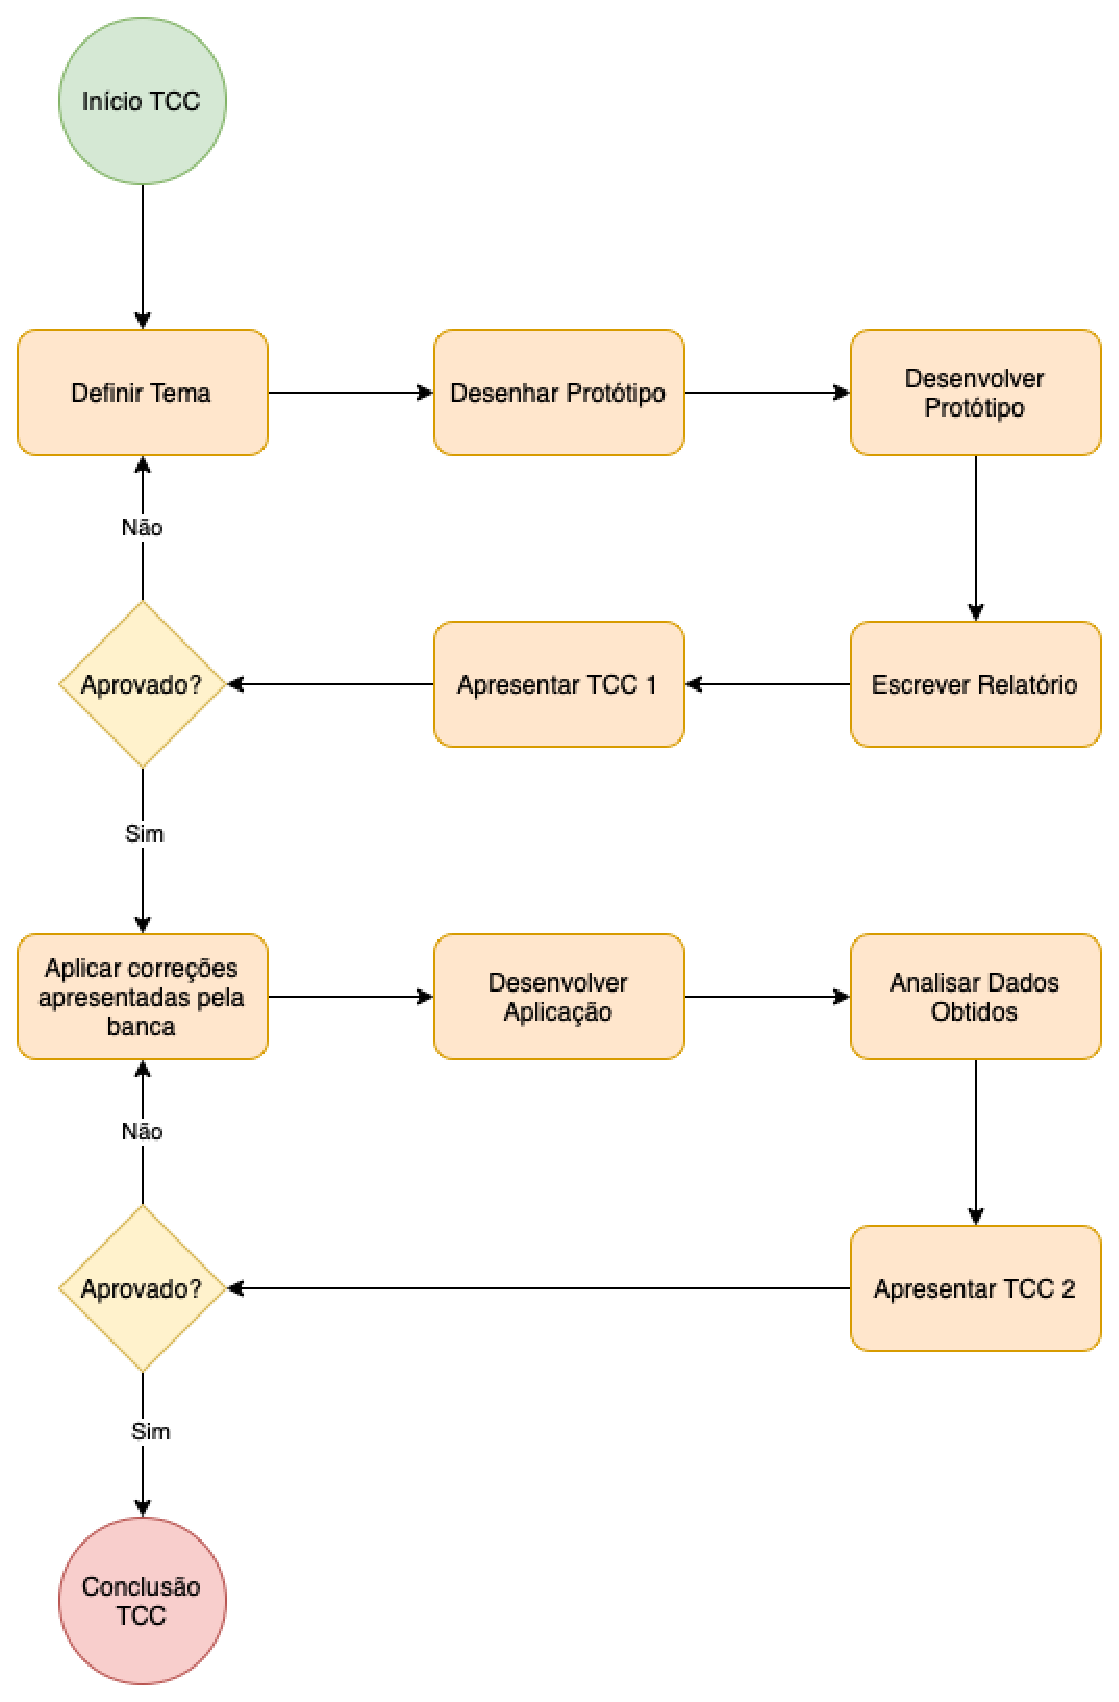
\includegraphics[keepaspectratio=true,scale=0.4]{figuras/metodologia.eps}
%     	\label{fig09}
%     \end{figure}

% \begin{itemize}
% 		\item \textbf{Definir tema}: atividade realizada e acompanhada pelo orientador. Essa etapa tem a finalidade de estabelecer qual a hipótese a ser explorada pelos autores.
% 		\item \textbf{Desenhar Protótipo}: atividade em que a arquitetura da solução é pensada e desenhada.
% 		\item \textbf{Desenvolver Protótipo}: atividade em que um protótipo da solução é desenvolvido, e a viabilidade do tema proposto é comprovada.
% 		\item \textbf{Escrever Relatório}: atividade onde o referencial teórico é coletado, as ideias da proposta são apresentadas, o protótipo é descrito, e os próximos passos são descritos.
% 		\item \textbf{Apresentar TCC 1}: atividade não realizada. Consiste na apresentação para avaliação da banca;
% 		\item \textbf{Aplicar correções apresentadas pela banca}: atividade não concluída. Sobre as adaptações sugeridas do trabalho de acordo com a análise feita pela banca avaliadora;
% 		\item \textbf{Desenvolver aplicação}: atividade iniciada. Envolve a implementação da aplicação proposta de acordo com o processo de desenvolvimento definido.
% 		\item \textbf{Analisar dados obtidos}: atividade não feita. Busca estudar os resultados da aplicação, analisando se a mesma cumpriu os objetivos do trabalho.
% 		\item \textbf{Apresentar TCC 2}: atividade não feita. A respeito da apresentação final do trabalho junto à banca.
% \end{itemize}

% \section{Metodologia de Desenvolvimento}

% O processo de desenvolvimento do \textit{software} proposto será realizado dentro das fases apresentadas no modelo BPMN, ilustrado na Figura \ref{fig10}. Cada etapa de desenvolvimento é executado segundo o fluxo de atividades abaixo:

% \begin{itemize}
% 		\item \textbf{\textit{Backlog} do produto}: é o artefato que procura agrupar todos os requisitos da aplicação entre outras tarefas necessárias para o desenvolvimento da aplicação;
% 		\item \textbf{Fazer}: atividades priorizadas e com o compromisso de ser desenvolvido. Pode-se alterar de acordo com a necessidade e andamento do projeto;
% 		\item \textbf{Fazendo}: atividades em desenvolvimento;
% 		\item \textbf{Revisão}: atividades finalizadas e que devem ser revisadas pelo orientador ou por outro desenvolvedor para melhorias, e
% 		\item \textbf{Feito}: atividades concluídas e que podem ser adicionadas à versão em produção do \textit{software}.
% \end{itemize}

%     \begin{figure}[!h]
%     	\centering
%     	\caption{Modelo BPMN do fluxo de desenvolvimento}
%     	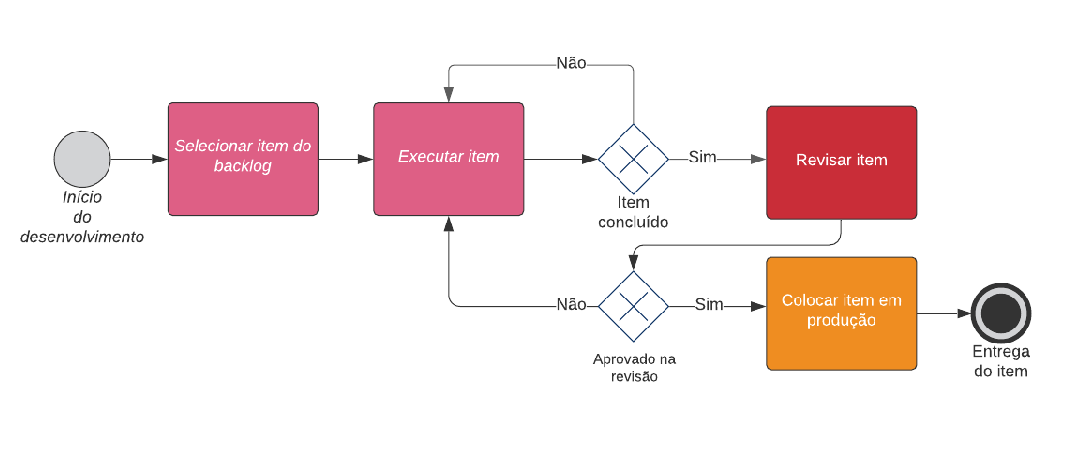
\includegraphics[keepaspectratio=true,scale=0.6]{figuras/fluxo_dev.eps}
%     	\label{fig10}
%     \end{figure}

% \section{Metodologia de Análise de Resultados}

% A pesquisa-ação assume "uma modalidade de pesquisa que não se ajusta ao modelo clássico de pesquisa científica, cujo propósito é o de proporcionar a aquisição de conhecimentos claros, precisos e objetivos" \cite{MetodoPesquisa}. Por isso, segue o fluxo que será usado para orientar a análise de resultados do presente projeto, ilustrado na Figura \ref{fig11}:

% \begin{itemize}
% 		\item \textbf{Coleta de dados}: absorver e abstrair dados através de cenários de uso planejados;
% 		\item \textbf{Análise e interpretação dos dados}: observar os dados coletados e interpretar os dados obtidos de forma empírica;
% 		\item \textbf{Plano de ação}: organização de uma ação para o problema alvo da analisado, e
% 		\item \textbf{Divulgação dos resultados}: documentar os resultados obtidos.
% \end{itemize}

%     \begin{figure}[!h]
%     	\centering
%     	\caption{Ciclo de pesquisa-ação}
%     	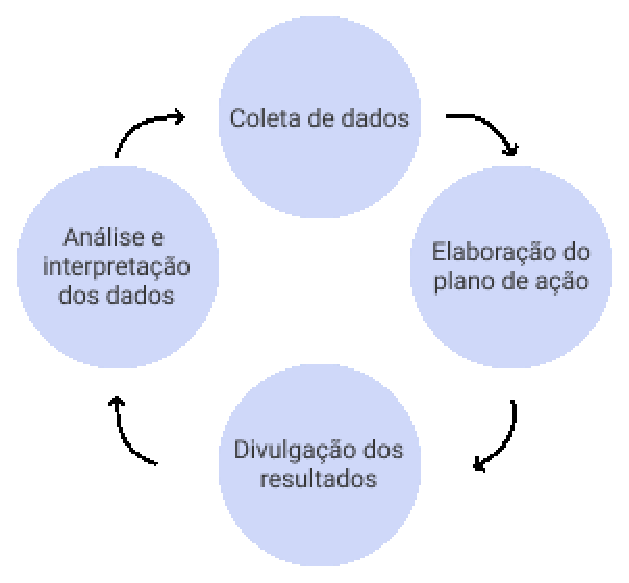
\includegraphics[keepaspectratio=true,scale=0.6]{figuras/ciclo_gil.eps}
%     	\label{fig11}
%     \end{figure}

% \section{Cronograma}

% A Tabela \ref{tab:cronograma_tcc} apresenta o cronograma de atividades executadas no TCC 1. Já a Tabela \ref{tab:cronograma_tcc2} acorda o cronograma preliminar de atividades previstas para serem realizadas no TCC 2.

% \begin{table}[!h]
%     \centering
%     \caption{Cronograma do Trabalho de Conclusão de Curso 1.}
%     \label{tab:cronograma_tcc}
%     \begin{tabular} {c|c|c|c|c|c}
%     \hline
%         \textbf{Atividade} & \textbf{Jul/2021} & \textbf{Ago/2021} & \textbf{Set/2021} & \textbf{Out/2021} & \textbf{Nov/2021} \\
%         \hline
%         Definir tema & X &  &  &  &  \\
%         \hline
%         Desenhar protótipo  &  X & &  &  &  \\
%         \hline
%         Desenvolver protótipo  &  & & X  &  &  \\
%         \hline
%         Escrever Relatório  &  &  &  &  X &  \\
%         \hline
%         Apresentar à banca   &  &  &  &  & X \\
%         \hline
%     \end{tabular}
%     \label{tab:cronograma_tcc}
% \end{table}

% \begin{table}[!h]
%     \centering
%     \caption{Cronograma do Trabalho de Conclusão de Curso 2.}
%     \label{tab:cronograma_tcc2}
%     \begin{tabular} {p{4cm}|c|c|c|c|c}
%     \hline
%         \textbf{Atividade} & \textbf{Jan/2022} & \textbf{Fev/2022} & \textbf{Mar/2022} & \textbf{Abr/2022} & \textbf{Mai/2022} \\
%         \hline
%         Aplicar correções & X &  &  &  &  \\
%         \hline
%         Desenvolver ferramenta  & X & X & X &  &  \\
%         \hline
%         Coletar e analisar resultados  &  &  &  & X &  \\
%         \hline
%         Apresentar à banca  &  &  &  &  & X \\
%         \hline
%     \end{tabular}
%     \label{tab:cronograma_tcc2}
% \end{table}

% \section{Considerações Finais do Capítulo}

% O presente capítulo apresentou todas as tomadas de decisão da metodologia do trabalho. Sendo assim, a metodologia de pesquisa deste trabalho pode ser  classificada como sendo uma abordagem qualitativa, com natureza aplicada, tendo o seu objetivo de se tornar uma pesquisa explicativa e o seu procedimento de pesquisa-ação. Finalmente, foram definidos os fluxos de desenvolvimento da aplicação e, igualmente, análise dos resultados.
